\chapter{Mesh Transformations}

This chapter discusses mesh transformations, i.e., locally update mesh by inserting a new vertex, or flips.

\section{Point insertion}

This section discusses the implementation of inserting a vertex. The Bowyer-Watson algorithm~\cite{Bowyer81, Watson81} is used to implement this. It also handles the insertion of hull vertex, i.e., the convex hull will be updated.

\begin{figure}
  \centering
  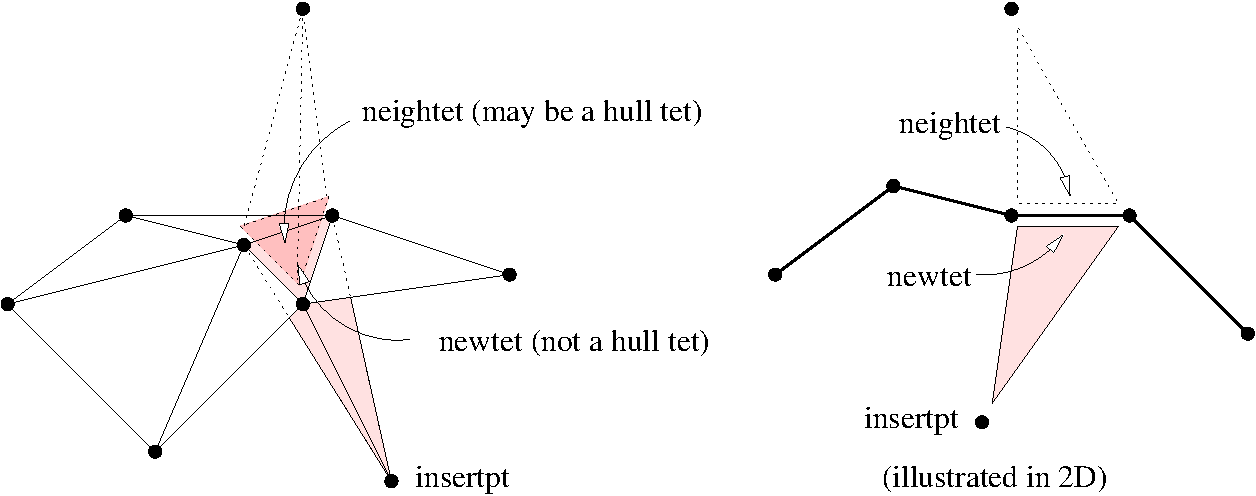
\includegraphics[width=0.9\textwidth]{../figs/bowyerwatson1}
\caption{Insert a interior vertex. Here {\tt insertpt} lies inside the convex hull.}
\label{fig:bowyerwatson1}
\end{figure}

\begin{figure}
  \centering
  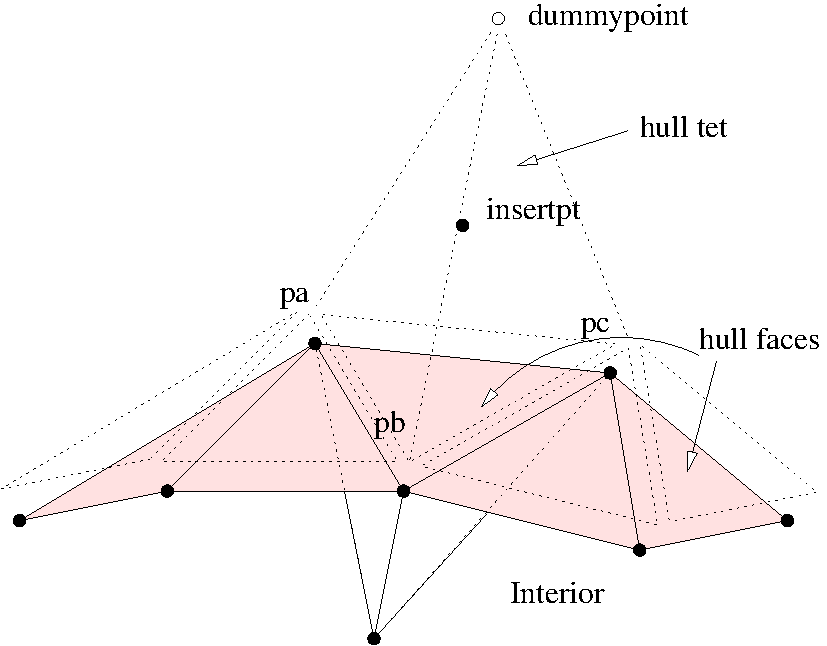
\includegraphics[width=0.6\textwidth]{../figs/inserthullvertex}
\caption{Insert a hull vertex. Here {\tt insertpt} lies outside the convex hull. }
\label{fig:inserthullvertex}
\end{figure}

\begin{figure}
  \centering
  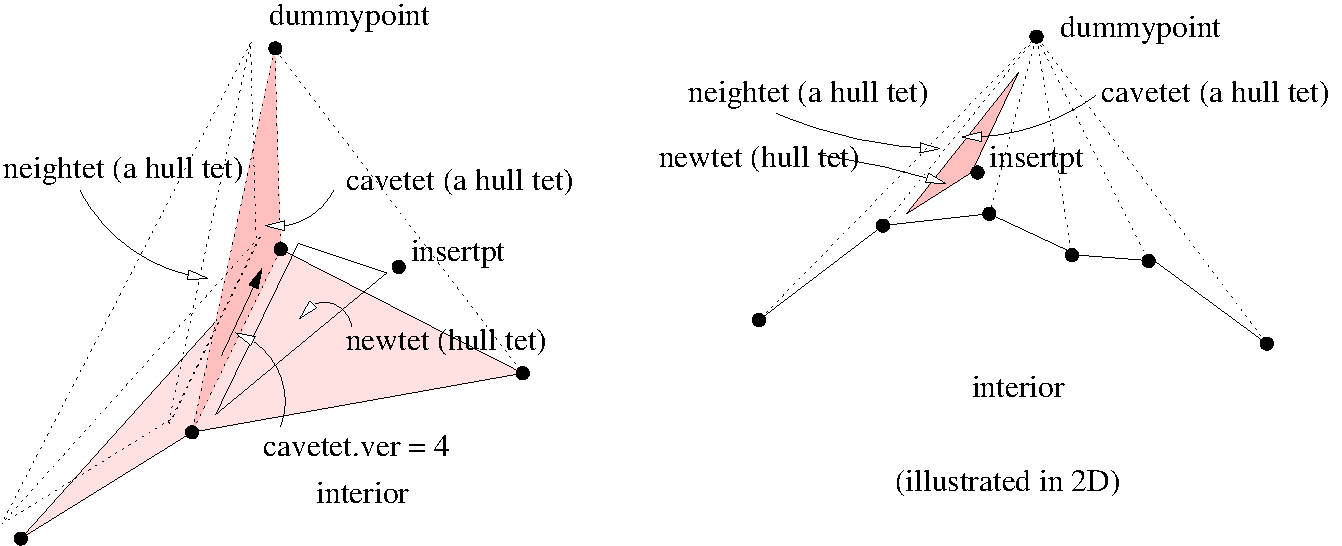
\includegraphics[width=1.0\textwidth]{../figs/bowyerwatson2}
\caption{Insert a hull vertex. Here {\tt insertpt} lies outside the convex hull. {\tt cavetet} is a hull tet, and it points to a side face whose apex is the {\tt dummypoint}. A {\tt newtet} is created on the base face of {\tt cavetet}, it is a hull tet.}
\label{fig:bowyerwatson2}
\end{figure}

\begin{figure}
  \centering
  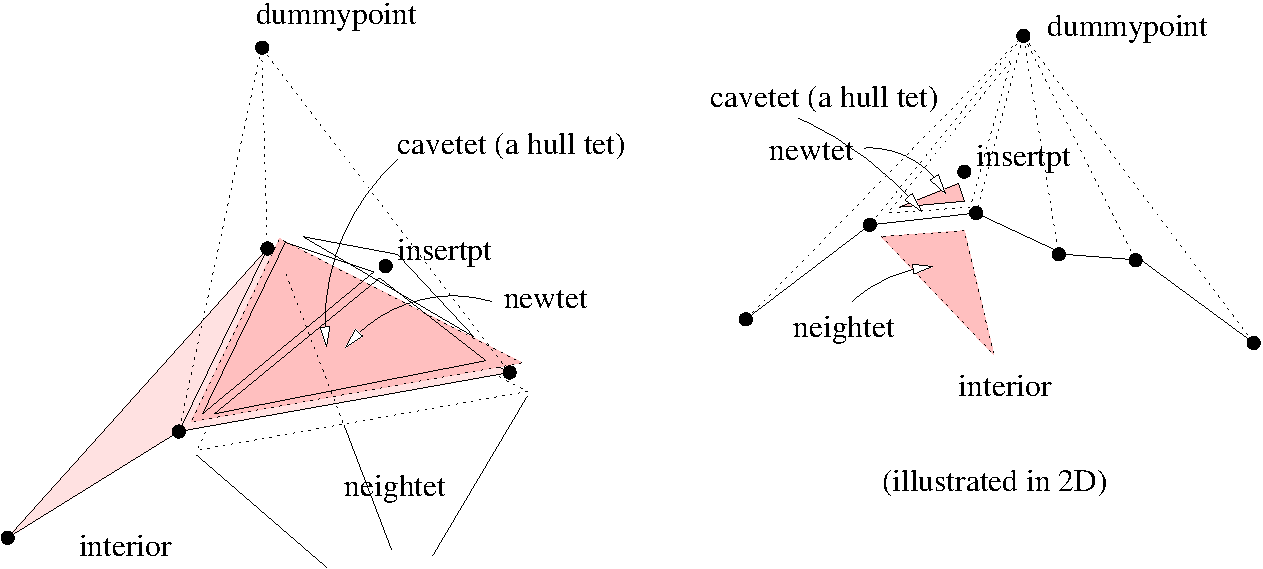
\includegraphics[width=1.0\textwidth]{../figs/bowyerwatson3}
\caption{Insert a hull vertex. Here {\tt insertpt} lies outside the convex hull. {\tt cavetet} is a hull tet, and it points to its base face which is visible by {\tt insertp}. A {\tt newtet} is created on the base face of {\tt cavetet}, it is not a hull tet.}
\label{bowyerwatson3}
\end{figure}
